\chapter{Trabajo Relacionado}

En este capítulo hablaremos sobre la variedad de expedientes clínicos electrónicos que pueden existir, desde un simple sistemasa clínico para un concultorio hasta un sistema formal para una unidad médica completa, aquí observares algunos que son los más utilizados de manera comercial y uno implementado en una unidad medica pública.

\section{Expediente Clínico Electrónico – ISSSTEMed}

En el 2007 el Expediente Clínico Electrónico ISSSTEMed es liderado por la Dirección Médica, redireccionando sus funcionalidades, teniendo como objetivo coadyuvar en la conformación de un Sistema de Salud Integrado. Está encaminado a implementar un sistema informático que permita agilizar, mejorar e integrar los procesos médico - administrativos del Instituto en sus tres Niveles de Atención. Fue conceptualizado como un Sistema de Registro Integral de la Atención Médica que recibe el derecho ambiente y que conecta a las diferentes áreas de la Unidad Médica. \cite{ISSTE}

\begin{center}
  \begin{minipage}{0.9\linewidth}
    \vspace{5pt}%margen superior
    {\small
    La Clínica Hospital ISSSTE Orizaba abre sus puertas para la realización del programa de capacitación de ISSSTEMED de administradores y personal médico de distintas unidades medicas del estado a cargo del Ing. Ricardo Villanueva Figueroa y la Dra. Nancy Berenice Morales Castro.
    Dicha capacitación se realizó el día  jueves 25 de Marzo del 2010 en el auditorio de las instalaciones de esta unidad médica, en punto de las nueve de la mañana, el objetivo fue la capacitación y reforzamiento de conocimientos y habilidades necesarias para el uso del programa ISSSTEMED (expedíente clínico electrónico).
    }
    \begin{flushright}
      (\author{Imágen del golfo.},
      \citeyearNP{http://imagendelgolfo.mx/resumen.php?id=164101}: 2010)
    \end{flushright}
      \vspace{5pt}%margen inferior de la minipage
  \end{minipage}
\end{center}

\begin{center}
  \begin{minipage}{0.9\linewidth}
    \vspace{5pt}%margen superior
    {\small
    La delegación de Veracruz tiene gran interés en que tanto personal médico como administradores se hagan responsables del sistema de cada unidad ya que de esta manera el expediente clínico de cada paciente podrá ser utilizado desde cualquier lugar.
    Dentro de la capacitación se dieron cita cerca 28 administradores del programa entre ellos médicos y demás personal administrativo de diferentes unidades como es el Hospital "Heroica Veracruz", Coatzacoalcos, Minatitlán, Cosamaloapan, Xalapa, Córdoba, Tuxpan, San Andrés Tuxtla, Acayucan, Tierra Blanca, Huatusco, Cerro Azul, Ciudad Alemán, Poza Rica, Martínez de la Torre, Naranjos y Orizaba.
    El administrador a nivel delegacional el ingeniero Villanueva Figeroa comentó acerca del programa: "Se pretende administrar los perfiles de las clínicas a manera que no existan estancamientos y sean rápidas las soluciones a los problemas del expediente".
    La Dra. Nancy Berenice Morales Castro puntualizó que espera que el programa ISSSTEMED arranque en el mes de junio o julio con Orizaba y Coatzacoalcos ya que: "para mi es como pasar de la era de piedra a la época de la comunicación" advirtió la doctora a cargo de este programa de capacitación.
    }
    \begin{flushright}
      (\author{Imágen del golfo.},
      \citeyearNP{http://imagendelgolfo.mx/resumen.php?id=164101}: 2010)
    \end{flushright}
      \vspace{5pt}%margen inferior de la minipage
  \end{minipage}
\end{center}


\subsection{Elementos de programación y desarrollo del sistema}
 Revisión y mantenimiento de los elementos de programación para garantizar el registro y procesamiento de información de las unidades médicas en operación y de nueva incorporación \cite{ISSTE}

\subsection{Aplicación}
 Fortalecimiento en la intercomunicación con otros sistemas (Afiliación y Vigencia, Abasto de Medicamentos y Cita Médica Telefónica e Internet.

\subsection{Acciones de mejora Fortalecimiento de la infraestructura tecnológica }
\begin{itemize}
  \item Diagnóstico de la red de telecomunicaciones.
  \item Reforzamiento de la red de telecomunicaciones.
  \item Liberación de anchos de banda conforme al programa de despliegue.
  \item Asegurar la alta disponibilidad del DATA CENTER.
  \item Migración de la nueva versión a la infraestructura de servidores con mayor capacidad. \ref{figura1}


\end{itemize}

\begin{figure}[h]
  \centering
  \label{figura1}
  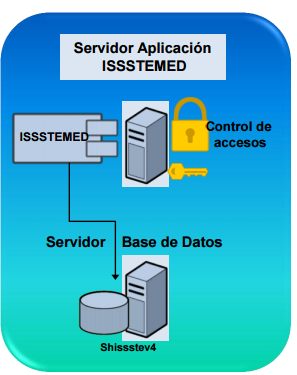
\includegraphics[scale=.35]{lib/assets/1}
  \caption{Servidor Aplicación ISSTEMED. (ISSSTE, 2010).}
\end{figure}


 %\subsection{Unidades implantadas}

%TABLA 1. Tabla de capacitaciones de servidores públicos. \cite{ISSTE}



\section{Virtualmedik}

\subsection{Expediente Clínico Electrónico}
Permite asegurar que los pacientes recibaExpediente Clínico Electrónicon el más oportuno, conveniente y eficiente cuidado de la salud, además mejora la productividad de los profesionales de la medicina. \cite{Villareal}

\subsection{Características}
Virtumedik es una aplicación que permite al médico organizar fácilmente toda la información clínica de sus pacientes a través de prácticamente de cualquier dispositivo con conexión a internet.
Diseño limpio: Interfaz adaptada al uso común de los médicos.
Accesible en todo lugar: Ten facilidad de movimiento y mejor servicio a tus pacientes.
Amigable y sencilla de usar: La curva de aprendizaje del ECE es corta y los beneficios enormes.
Cumple con la NOM 024, Ten todo en regla y listo para usarse de manera legal y correcta desde el primer momento.
100\% Confidencial: Tu información y la de tus pacientes está protegida por estándares internacionales de seguridad informática.
Agenda Multiconsultorio: Porque sabemos cómo es el trabajo de los profesionales de la salud, el multiconsultorio es un plus necesario.\cite{Villareal}
\subsection{Descarga de la aplicación:}
\begin{itemize}
  \item En su unica version para iPad.
  \ref{figura2}
\end{itemize}

\begin{figure}[h]
  \centering
  \label{figura2}
  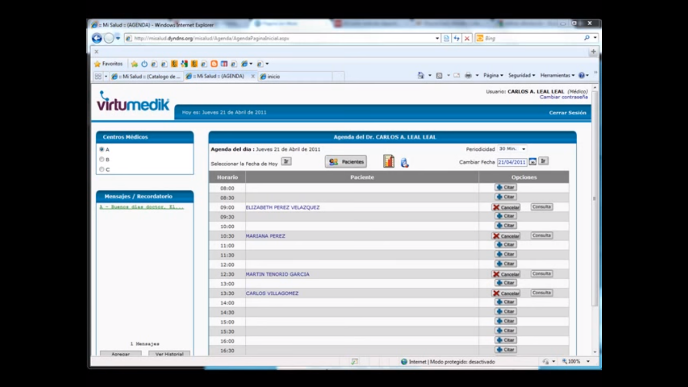
\includegraphics[scale=1]{lib/assets/2}
  \caption{Interface de virtualmedik (www.virtualmedik.com, S.F).}
\end{figure}

\section{MediSel}
Empresa mexicana creada en el año 2001, dedicada al desarrollo de soluciones tecnológicas para el área médica.
Ofrecemos el servicio de Expediente Clínico Electrónico totalmente en la nube desde el año 2007. En el mes de junio del año 2012, participaron en el proceso de revisión ante la secretaría de Salud Federal, validando el cumplimiento de la NOM-004-SSA3-2012.
Actualmente el servicio es usado por más de 1,500 médicos de toda la república mexicana \cite{Villareal}
\subsection{Características}
Importa con un clic los signos vitales que el asistente o enfermera le tomó al paciente. Reciba alertas de interacciones medicamentosas y alergias. Reportes estadísticos de los pacientes con algún diagnóstico o tratamiento. La red de 30 servidores MediSel, distribuidos en centros de datos en San Antonio, California, Florida y Virginia le garantizan el 100\% de confiabilidad y disponibilidad de la información. Por ser un sistema totalmente en la nube, MediSel puede ser configurado para trabajar en diferentes esquemas de trabajo, sin que el médico o administrador de la clínica o centro de atención médica tenga que invertir en procesos de implementación del sistema, servidores locales, ni personal técnico \cite{Villareal}
Dra. Gabriela Villarreal Levy, Ex Directora del Proyecto Nacional del Expediente Clínico Electrónico 2007-2011 de la Secretaría de Salud Federal.

\subsection{Esquemas de trabajo en los que puede ser configurado MediSel}

\subsubsection{Un consultorio médico.}
Este es el modo básico de trabajo, el médico y su asistente. La asistente con sus credenciales colabora en la administración de la información, teniendo un acceso limitado a los módulos del sistema. El médico desde cualquier dispositivo con acceso a Internet, accede al sistema, estando físicamente en el consultorio, o en una ubicación remota.\cite{esquemas} \ref{figura3}
\begin{figure}[h]
  \label{figura3}
  \centering
  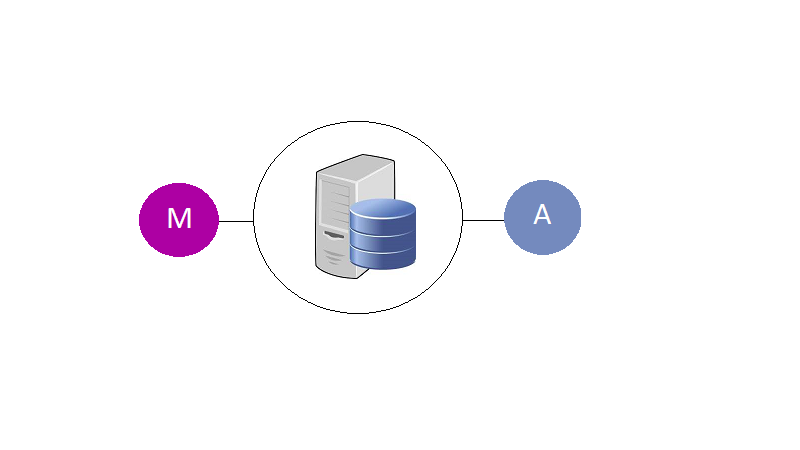
\includegraphics[scale=.35]{lib/assets/3}
  \caption{Un consultorio medico}
\end{figure}




\subsubsection{Varios consultorios médicos.}
El médico puede crear sin costo alguno todas las cuentas que necesite para sus asistentes. Este esquema es muy común para médicos que tienen más de una asistente en el mismo consultorio o varias asistentes en diferentes consultorios. Por ejemplo, el médico puede dar consultas lunes y miércoles en el consultorio de un hospital y martes, jueves y viernes dar consultas en otro consultorio. En ambos consultorios que pueden estar físicamente muy distantes, las asistentes colaboran administrando la misma agenda de citas y el registro de pacientes \cite{esquemas} \ref{figura4}

\begin{figure}[h]
  \label{figura4}
  \centering
  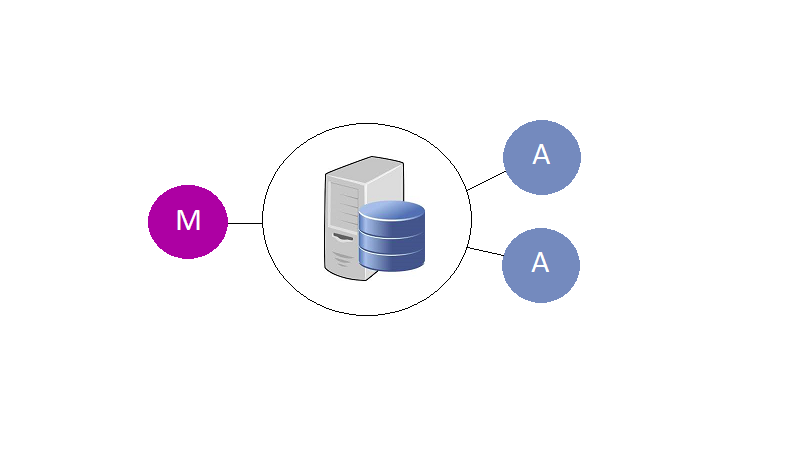
\includegraphics[scale=.35]{lib/assets/4}
  \caption{Varios consultorios médicos.}
\end{figure}



\subsubsection{Clínica o Centro de Atención Médica.}
Este esquema aplica para una clínica o centro de atención médica donde el expediente clínico del paciente se comparte entre varios médicos. También aplica para grupos de médicos que físicamente se encuentran distantes pero que comparten los mismos pacientes. Para esta configuración se crean usuarios con permisos especiales que administran todos los usuarios del grupo a través de la plataforma de administración para grupos. \cite{esquemas} \ref{figura5}

\begin{figure}[h]
  \label{figura5}
  \centering
  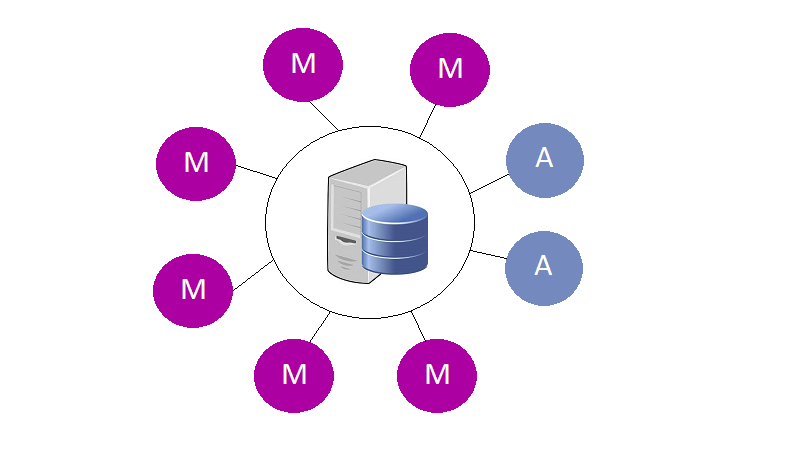
\includegraphics[scale=.35]{lib/assets/5}
  \caption{Clínica o Centro de Atención Médica.}
\end{figure}


\subsubsection{Red estatal o nacional de salud.}
MediSel puede ser configurado para redes de salud médica a nivel estatal o nacional, donde se pueden integrar clínicas o centros de atención médica. La información estadística generada por todos los integrantes de la red puede ser consolidada y consultada en tiempo real. \cite{esquemas} \ref{figura6}

\begin{figure}[h]
  \label{figura6}
  \centering
  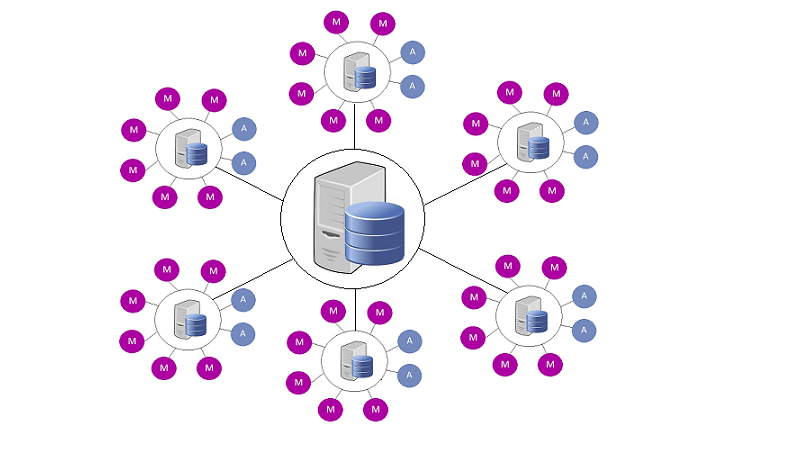
\includegraphics[scale=.35]{lib/assets/6}
  \caption{Red estatal o nacional de Salud.}
\end{figure}







\section{Elex}
\begin{center}
  \begin{minipage}{0.9\linewidth}
    \vspace{5pt}%margen superior
    {\small
Es un software orientado a MEDICOS, odontólogos, psicólogos, centros médicos, consultorios particulares. Este software contiene módulos de gestión para el manejo de todos los apartados de las historias clínicas, además de directorio, herramientas como calculadora, enlace a páginas de interés de ciencias de la salud, presupuestos, estadísticas, etc. \ref{figura12}
    }
    \begin{flushright}
      (\author{Elex},
      \citeyearNP{http://www.elex.com.mx:9080/elex2.0}: 2010)
    \end{flushright}
      \vspace{5pt}%margen inferior de la minipage
  \end{minipage}
\end{center}

El sistema corre en un servidor dedicado y tiene acceso por internet para darle la portabilidad necesaria y lo pueda usar desde cualquier parte del mundo.
\subsection{Características:}
  \begin{itemize}
    \item Permite introducir usuarios y contraseñas.
    \item Identificaciones de pacientes con foto.
    \item Permite agregar fotografía clínica a los historiales.
    \item Manejo e impresión de recetas.
    \item Reporte de historiales.
    \item Agenda de citas.

  \end{itemize}

  \begin{center}
    \begin{minipage}{0.9\linewidth}
      \vspace{5pt}%margen superior
      {\small
      Base de datos anexa para guardar los fármacos que más usa
      Los datos de fármacos pueden ser utilizadas para impresión de recetas
      Búsquedas fáciles pero poderosas en todos los datos
      Copia de respaldo automática
      Archivo de ayuda disponible
      Cumple con la norma NOM-168-SSA1-1998
      NOM-024-SSA3-2010 (expedientes clínicos electrónicos) *En Acreditación.
      }
      \begin{flushright}
        (\author{Elex},
        \citeyearNP{http://www.elex.com.mx:9080/elex2.0}: 2010)
      \end{flushright}
        \vspace{5pt}%margen inferior de la minipage
    \end{minipage}
  \end{center}

\subsection{Ventajas:}


\begin{center}
  \begin{minipage}{0.9\linewidth}
    \vspace{5pt}%margen superior
    {\small
    \begin{itemize}
      \item Flexibilidad: Requiere los mínimos conocimientos de computación.
      \item Seguridad: Únicamente los usuarios registrados pueden tener acceso. 
      \item Cuenta con el debido protocolo de ingreso a la aplicación.
      \item Velocidad: Economiza el tiempo de búsqueda del expediente tradicional.
      \item Almacenaje: Compuesto de una base de datos electrónica capaz de almacenar una enorme cantidad de información más que sistemas tradicionales.
      \item Accesibilidad: Nos permite tener acceso a la información del paciente en el momento deseado.
    \end{itemize}
    }
    \begin{flushright}
      (\author{Elex},
      \citeyearNP{http://www.elex.com.mx:9080/elex2.0}: 2010)
    \end{flushright}
      \vspace{5pt}%margen inferior de la minipage
  \end{minipage}
\end{center}


\subsection{Beneficios:}

\begin{center}
  \begin{minipage}{0.9\linewidth}
    \vspace{5pt}%margen superior
    {\small
    \begin{itemize}
      \item Incremento en la productividad.
      \item Reducción de costos.
      \item Prevención de errores en diagnósticos.
      \item Información centralizada.
      \item Seguridad de la información.
      \item Mayor calidad en la atención al paciente.
      \item Expediente clínico ordenado y legible.
      \item Accesibilidad a la información.
    \end{itemize}
    }
    \begin{flushright}
      (\author{Elex},
      \citeyearNP{http://www.elex.com.mx:9080/elex2.0}: 2010)
    \end{flushright}
      \vspace{5pt}%margen inferior de la minipage
  \end{minipage}
\end{center}



\section{Medyca}
Es uno de los principales Centros médicos, con una organización ágil que se identifica por su alto compromiso en la prestación de salud integral, personalizado, con sentido ético y calidez humana, superando en todo momento sus expectativas de servicio, calidad y mejoramiento continuo siempre a la vanguardia. \cite{mediesel}

\subsection{Características}
\begin{itemize}
  \item Cuenta con una de las más avanzadas tecnologías médicas, el Expediente Clínico Electrónico Medyca está a la vanguardia en el desarrollo e implementación del sistema informático para el intercambio de información clínica con la creación del Expediente Clínico Electrónico. Esta avanzada tecnología nos permite contar con el historial médico de cada paciente compartida al instante, cumpliendo con los principios de disponibilidad, integridad y confidencialidad, de acuerdo a la normatividad vigente. \cite{mediesel}

\item Cuando un paciente se atiende, forzosamente genera información clínica importante para su historial. Antes esa información se imprimía y se archivaba en un fólder, la cual permanecía en las instalaciones donde recibió dicha atención.\cite{mediesel}

\item Ahora mediante el Expediente Clínico Electrónico se podrá brindar información más completa a los médicos en sus diferentes especialidades y habilitar la comunicación al instante entre distintas instalaciones, pudiendo conocer la información clínica del paciente desde el cualquier unidad de atención, hospital o inclusive de diferente ciudad, las 24 horas del día cualquier día de la semana. \cite{mediesel}
\end{itemize}

\subsection{Interacción}
El Expediente Clínico Electrónico del paciente, interactúa también con sistemas como los de:
\begin{itemize}
  \item Laboratorio
  \item Patología
  \item Radiología
  \item Farmacia y Hospitales
\end{itemize}

De tal manera que la solicitud de estudios llegue vía electrónica y los resultados se integren de inmediato al expediente, o de la Farmacia de modo que se prepare anticipadamente el surtido de la receta, imprimiendo a la vez etiquetas con las indicaciones de cada medicamento para evitar confusiones al paciente.
Así como disponer en los Hospitales toda la información médica importante del paciente para la toma de decisiones tanto diagnosticas como terapéuticas. \cite{mediesel} \ref{figura7}
\begin{figure}
  \label{figura7}
  \centering
  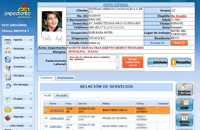
\includegraphics[scale=1]{lib/assets/7}
  \caption{Interface del Expediente Clínico Electrónico Medyca.}
\end{figure}
